% !TEX root = main.tex
%
% Introduction
%
Various extensions of language models have been proposed for handling infinite alphabets.
%words carrying data values in an infinite domain (e.g. integers) e.g. data processing
Some automata 
%\reviews{1) and grammar with storage?}
with memory extensions
allow restricted storage and comparison of input symbols
%and correspond with logics,
(see~\cite{Segoufin06csl} for a survey).
\florent{register: skip refs and details, add Mikolaj recent}
They use pebbles for marking positions~\cite{NevenSchwentickVianu04FSMinfinite},
registers~\cite{KaminskiFrancez94},
or %computations in 2 steps
separate computation on subsequences
with the same attribute values~\cite{Bojanczyk11FO2}. % data words automata.
%
%for the and verification of infinite state systems
%(model checkers: alphabet = long bit-vectors)
%...For the representation of  in model checking, verification and
%
Moreover, automata at the core of model checkers
compute on input symbols represented by large bitvectors~\cite{Vardi07ciaa} %\cite{BaierKatoen08MC}
%(sets of assignments of Boolean variables) %propositional variables)
and, in practice,  %implementation
each transition accepts a set of such symbols (instead of an individual symbol),
represented by Boolean Formulas or Binary Decision Diagrams.
%
Following this idea, % and generalizing,
in symbolic automata (\SA)~\cite{Veanes12symbolic,dAntoniVeanes17CAV,dAntoni21CACM},
transitions are guarded by predicates over large or infinite domains.
With appropriate closure conditions on the sets of such predicates, % (alphabet theories),
all the good properties enjoyed by automata over finite alphabets are preserved.
The ability to compare input symbols of \SA is quite restricted compared to the 
former automata with memory. 
It can however be extended with the addition of a stack~\cite{dAntonyAlur14SVPDA}.

Other extensions of language models  %(automata and grammars)
assign one weight value to every input~\cite{Droste09handbook}.
%help in dealing with non-determinism
This is useful for the quantitative modelling of
\eg probabilistic or stochastic recursive programs, %( for pushdown models),
quantitative database queries, or semi-structured data, % (in infinite domains), 
as well as for the verification of quantitative properties about 
\florent{quantitative reasoning/verification on programs}
quality measures, resource-consumption, distance metrics, probabilistic guarantees, \etc
%
In the context of parsing, when grammars return weight values, 
it is possible to rank derivations (and \emph{abstract syntax trees})
in order to select a best one (or $n$ bests),
%\florent{= "weighted parsing"}
\eg in case of ambiguity~\cite{Goodman99SemiringParsing,Nederhof03weightedParsing,MorbitzVogler19weighted-parsing}.
%This is roughly the principle of \emph{weighted parsing} approaches
%\reviews{1) jump from automata to grammars is uneasy and not really necessary}
% for which there may exist several derivations yielding one input word.
%
In \emph{weighted language models}
like \eg probabilistic context-free grammars % (CFG),
and weighted automata (\WA)~\cite{Droste09handbook},
a weight is associated to each transition rule, % production rule
and the weights of the rules involved in a computation are combined with an
associative product operator~$\otimes$. % to yield the weight of a whole computation.
%\reviews{1) AST for grammar, run for WA}
A second operator~$\oplus$
is moreover used to resolve the ambiguity raised by the existence
of several (in general exponentially many) computations on a given input.
Typically, $\oplus$ selects the best of two weight values.
%Intuitively,~$\oplus$ selects, or ranking, the syntax trees.
The weight domain, equipped with these two operators is typically 
a \emph{semiring} %$\Semiring$
where $\oplus$ can be extended to infinite sums,
%\cite{Eilenberg74automata}
such as the Viterbi semiring and the tropical min-plus algebra% % see Figure~\ref{fig:semirings}.
%of domain $\mathbb{R}^+ \cup \{ +\infty\}$,
%where $\oplus$ is min and $\otimes$ is plus .
%by ranking
%making the weight domain a semiring.
%Some efficient specialized parsing algorithms~\cite{Huang05kbest} have been proposed in this context
%% models represented as hypergraphs \cite{Huang05kbest}
%in order to compute the $n$ best syntax trees of a given input word without having to enumerate them all.
%Generally based on dynamic programming, these algorithms rely on
%additional algebraic properties of~$\Semiring$.
%-- see \eg~\cite{Huang05kbest} for some NLP applications.
%The extraction of $n$ best list is useful
%the problem: quantitative parsing or symbolic parsing
%of parsing of words over infinite input alphabet.

In this paper, we present some results for 
\emph{Symbolic Weighted} finite states language models %(\swM) 
generalizing the Boolean guards of~\SA %in transitions
to functions into an arbitrary semiring, 
and also the~\WA, by handling infinite alphabets (Figure~\ref{fig:hierarchy}).
%
The models considered are also 
%\SWA and \SWVPA are both 
particular cases of the very general class of 
Weighted Symbolic Automata with Data Storage~\cite{Herrmann16dlt,Herrmann20phd}, 
using appropriate storage types.
%with special data storage types...
%\florent{Both WA and SA generalized by \cite{Herrmann16dlt,Herrmann20phd}...}
%\reviews{cite \cite{Herrmann16dlt,Herrmann20phd}}

\begin{figure}
\centering
\begin{tikzpicture}
\node (SWADS) at (3.0,5.0) {%
  \(
  \begin{array}{c}
  \mathsf{SWADS}\,\mbox{\cite{Herrmann16dlt,Herrmann20phd}}
  \end{array}
  \)
};
%
\node (SWA) at (0,3.4) {%
  \(
  \begin{array}{c}
  \mathsf{SWA}: \Sigma_{\mathsf{inf}}^* \to \mathbb{S}\\
  q \xrightarrow{\phi} q', \phi : \Sigma_\mathsf{inf} \to \mathbb{S}
  \end{array}
  \)
};
%
\node (WA) at (-1.8,1.7) {%
  \(
  \begin{array}{c}
  \mathsf{WA}\,\mbox{\cite{Droste09handbook}}: \Sigma_{\mathsf{fin}}^* \to \mathbb{S}\\
  q \xrightarrow{a, w} q', a \in \Sigma_\mathsf{fin}, w \in \mathbb{S}
  \end{array}
  \)
};
%
\node (SA) at (1.8,1.7) {%8
  \(
  \begin{array}{c}
  \mathsf{SA}\,\mbox{\cite{Veanes12symbolic,dAntoni21CACM}}: \Sigma_{\mathsf{inf}}^* \to \mathbb{B}\\
  q \xrightarrow{\phi} q', \phi : \Sigma_\mathsf{inf} \to \mathbb{B}
  \end{array}
  \)
};
%
\node (NFA) at (0,0) {%
  \(
  \begin{array}{c}
  \mathsf{FA} : \Sigma_{\mathsf{fin}}^* \to \mathbb{B}\\
  q \xrightarrow{a} q', a \in \Sigma_\mathsf{fin}
  \end{array}
  \)
};
%
\node (VPA) at (5.6,0) {%
  \(
  \mathsf{VPA}\,\mbox{\cite{AlurMadhusudan09nested}}
  \)
};
%
\node (WVPA) at (4.6,1.7) {%
  \(
  \mathsf{WVPA}\,\mbox{\cite{Mathissen08weighted,Caralp12VPAmult}}
  \)
};
%
\node (SVPA) at (6.6,1.7) {%
  \(
  \mathsf{SVPA}\,\mbox{\cite{dAntonyAlur14SVPDA}}
  \)
};
%
\node (SWVPA) at (5.6,3.4) {%
  \(
  \mathsf{SWVPA}
  \)
};
%
\draw[->] (NFA)--(WA);
\draw[->] (NFA)--(SA);
\draw[->] (WA)--(SWA);
\draw[->] (SA)--(SWA);
\draw[->] (SWA)--(SWADS);
\draw[->] (VPA)--(WVPA);
\draw[->] (VPA)--(SVPA);
\draw[->] (WVPA)--(SWVPA);
\draw[->] (SVPA)--(SWVPA);
\draw[->] (SWVPA)--(SWADS);
%\begin{array}{c} \mathsf{NFA} : \Sigma^* \to \mathbb{B} \end{array}
\end{tikzpicture}
\caption{Classes of Symbolic/Weighted Automata.
Here, $\Sigma_\mathsf{fin}$ and $\Sigma_\mathsf{inf}$ denote finite/countable alphabets,
$\mathbb{B}$  the Boolean algebra,
$\mathbb{S}$ a commutative semiring.
$q \xrightarrow{\dots} q'$ is a transition between states $q$ and $q'$.}
\label{fig:hierarchy}
\end{figure}
%
%This approach is close to the case of
%Symbolic Automata (SA)~\cite{dAntoniVeanes17CAV,dAntoni21CACM},
%except that the domain for weight values is not restricted to be Boolean,
%like for the guards in the rules of SA,
%but can be an arbitrary commutative semiring (assuming some restrictions).

\noindent
In short, a transition rule $q \xrightarrow{\phi} q'$ of a SW automaton, 
from state $q$ to $q'$,
%\florent{c'est un résumé de la Fig. \ref{fig:hierarchy}}
%input symbols are variables, %(parameters)
is labeled by a function~$\phi$ associating to every input symbol~$a$, a weight value~$\phi(a)$
in a semiring~$\Semiring$.
%
The models studied are: 
symbolic-weighted automata (\SWA),
defining series over infinite alphabets, 
transducers (\SWT), 
defining distances between finite words over infinite alphabets, % following~\cite{Mohri03ijfcs}.
and pushdown automata with a visibility restriction~\cite{AlurMadhusudan09nested} (\SWVPA),
operating sequentially on %\emph{nested words}~\cite{AlurMadhusudan09nested},
words structured with markup symbols (parentheses) and describing linearizations of trees.
%A \SWVPA $A$ associates a weight value $A(t)$ % \in \Semiring$
%to a given nested word $t$, which is itsef the linearization of a weighted AST. %representing a parse tree.
%
The main contributions of this paper are:
%\reviews{1) not $i$! see response.txt}
%($i$)~the introduction of automata, \SWA, transducers, \SWT (Section~\ref{section:SWA}),
%and visibly pushdown automata \SWVPA (Section~\ref{sec:SWVPA}),
%generalizing the corresponding classes of symbolic and weighted models,
%for the weighted computation on (nested) words over infinite alphabets;
($i$)~the construction à la Bar-Hillel Perles Shamir of a \SWA
     computing a \SWT-defined distance between a \SWA input language and a word (Section~\ref{section:SWA}), 
($ii$)~closure results for \SWVPA, 
($iii$)~a polynomial best-search algorithm for \SWVPA (Section~\ref{sec:SWVPA}). %(Section~\ref{sec:best})
% a framework for parsing over infinite alphabets,
Moreover, we present in Section~\ref{sec:parsing} an 
($iv$) application to the problem of weighted parsing over infinite input alphabets, 
called \emph{SW-parsing}. 
%
The goal of this problem is, given an input word~$s$, 
to find~$t$ minimizing the distance, in the sense of~\cite{Mohri03ijfcs}, 
$T(s, t) \otimes A(t)$, where $T$ is a \SWT and $A$ a \SWVPA.
The notion of transducer-based distances allows to consider 
different infinite alphabets for the input $s$ and output $t$.
Moreover, the use of \SWVPA permits to consider output $t$ in the form of a (nested) word, instead of a tree.
%technical convenience
%the SW models are integrated in a uniform framework.
\emph{SW-parsing} is solved with the Bar-Hillel construction~\cite{NederhofSatta03ParsingIntersection} 
%\cite{GruneJacobs08parsing}
of a \SWVPA $B$ such that, for all~$t$, $B(t) = T(s, t) \otimes A(t)$
and the application of a best-search procedure to this automaton $B$.
% reduction to the shortest distance in graphs~\cite{Mohri02semiring,Huang05kbest}.

%Like weighted-parsing methods~\cite{Goodman99SemiringParsing,Nederhof03weightedParsing,MorbitzVogler19weighted-parsing},
%\reviews{1) WARNING: \cite{MorbitzVogler19weighted-parsing} incomparable to our def. weighted parsing}

%Parsing is the problem of structuring a linear representation
%(a finite word) according to a language model. % (a formal grammar). % natural language, programming language,

Context-free parsing approaches~\cite{GruneJacobs08parsing}
generally assume a finite and reasonably small input alphabet. %models and algorithms
%Such a restriction makes perfect sense in the context of
%NLP tasks such as constituency parsing, 
%compilers or interpreters for programming languages.
Considering large or infinite alphabets can however be of
practical interest when dealing with large characters encodings such as UTF-16~\cite{dAntoni21CACM}.
\florent{applis à la Fossacs chez Veanes et al?}
% processing strings in \eg for vulnerability detection in Web-applications~\cite{dAntoni21CACM},
%We believe that these results could also be useful 
It is also true in the context of automata-based quantitative verification,  %of systems processing %analysis of 
\eg when dealing with data streams, 
serialization of structured documents~\cite{Segoufin06csl,NevenSchwentickVianu04FSMinfinite},
or timed execution traces~\cite{Bouyer03algebraic}.

% algebraic definition of a class of data languages
% (notion of monoid recognizability, based on registers, comparable to Bojancszik et al. data words)

The latter case is related to a motivation  of  the present work: \florent{idem}
automated music transcription. Representations capturing music performances
are essentially linear~\cite{Selfridge-Field97beyondMIDI};
%audio files or the widely used MIDI format %\cite{MIDIfile}.
they ignore the hierarchical structures that frame the
conception of music, at least in the Western area. 
These structures, on the other hand, are present, either explicitly  or implicitly,
in Common Western Music Notation~\cite{Gould11Notation}:
%in music notation~\cite{Gould11Notation}:
Music scores are partitioned in measures,
measures in beats, and beats can be further recursively divided.
It follows that written music events do not occur at arbitrary timestamps,
but respect a discrete partitioning of the timeline incurred by
these recursive divisions.
The \emph{transcription problem} takes
as input a linear performance (audio or MIDI) and aims at re-constructing
structured notation, 
by mapping input events to this hierarchical rhythmic space.
It can therefore be stated as a parsing problem
over an infinite alphabet of timed events~\cite{foscarin:hal-01988990}.

%In expressiveness, they are equivalent to weighted CFG.
%and can be used in a general approach for parsing over infinite input alphabets.
%
%Let $A$ be a \SWVPA, associating $A(w) \in \Semiring$
%to a given a nested word $w$ (representing a parse tree),
%and let a \SWT compute a distance $d$, in $\Semiring$,
%between 2 strings over respectively an infinite input alphabet and the
%same (infinite) alphabet of $A$.
%Then, the problem of Symbolic Weighted Parsing is,
%given an input string $s$, to find a nested word $w$ minimizing
%(according to the ranking defined by $\oplus$)
%the distance $d(s, w) \otimes A(w)$ between $s$ and $A$,
%as defined in~\cite{Mohri03ijfcs}.

% First one general edit-distance is defined by a weighted word
% transducer~\cite{Mohri}
% %Symbolic automata transducers are extended models~\cite{VeanesdAntoniJACM}
% %dealing with infinite set of input symbols...
% value in a semiring...


\florent{expressiveness: VPA have restricted equality test.
        comparable to pebble automata? $\to$ conclusion}
        
        
\begin{example}%[Running example]
\label{ex:running}
We illustrate our approach with a very simplified %toy
running example of \emph{music transcription}:
a given input \emph{timeline} of musical events
from an infinite alphabet $\Sigma$,
is parsed into a structured music score.
Input events of $\Sigma$
are pairs $\mu \tstamp{\tau}$, where $\mu$ is a
MIDI key number~\cite{Selfridge-Field97beyondMIDI}, %\cite{MIDIfile}
and $\tau \in \mathbb{Q}$ is a timestamp in seconds.
Such inputs typically correspond
to the recording of a live performance, 
\eg~$I = 69\tstamp{0.07},
	     71\tstamp{0.72},
    	 73\tstamp{0.91},
	     74\tstamp{1.05},
	     76\tstamp{1.36},
	     77\tstamp{1.71}$. % over interval $[0,2[$,

The output of parsing is a sequence of
timed symbols $\nu\tstamp{\tau'}$ in an alphabet $\Delta$,
%events (or \emph{notes})
%in Common Western Music Notation (CWMN)~\cite{Gould11Notation}
where $\nu$  represents
an \emph{event} (or \emph{note}),
specified by its \emph{pitch name}
(\eg, $\mbox{\footnotesize A4}$, $\mbox{\footnotesize G5}$, \etc.),
an event \emph{continuation} (symbol `$-$`, see Example~\ref{ex:SWT}),
or a \emph{markup} (opening or closing parenthesis). %(\emph{parenthesis}),
The temporal information $\tau'$ 
is either a time interval, for the opening parentheses
(representing the duration between the parenthesis 
 and the matching closing one), 
or a timestamp, for the other symbols.
The time points in $\tau'$ belong to a rhythmic ``grid'' obtained from recursive divisions:
whole notes ($\musWhole$) split in halves ($\musHalf$), halves
in quarters ($\musQuarter$), eights ($\musEighth$), \etc.
%
For instance, the output score
\includegraphics[scale=0.35,trim=0 5mm 0 0]{pictures/ex1.pdf},
  %\includegraphics[scale=0.20]{pictures/score5.png},
corresponds to a hierarchical structure
that can be linearized as the sequence
$O =$
$\ccall{\mathsf{m}}\tstamp{[0,1]}$,
$\ccall{2}\tstamp{[0,1]}$,
$\mbox{\footnotesize A4}\tstamp{0}$,
$\ccall{2}\tstamp{[\frac{1}{2},1]}$,
$-\tstamp{\frac{1}{2}}$,
$\ccall{2}\tstamp{[\frac{3}{4},1]}$,
$\mbox{\footnotesize B4}\tstamp{\frac{3}{4}}$,
$\mbox{\footnotesize C$\sharp$5}\tstamp{\frac{7}{8}}$,
$\creturn{2}\tstamp{1}$,
$\creturn{2}\tstamp{1}$,
$\creturn{2}\tstamp{1}$,
$\creturn{\mathsf{m}}\tstamp{1}$,
$\ccall{\mathsf{m}}\tstamp{[1,2]}$,
$\ccall{3}\tstamp{[1,2]}$,
$\mbox{\footnotesize D5}\tstamp{1}$,
$\mbox{\footnotesize E5}\tstamp{\frac{4}{3}}$,
$\mbox{\footnotesize F5}\tstamp{\frac{5}{3}}$,
$\creturn{3}\tstamp{2}$,
$\creturn{\mathsf{m}}\tstamp{2}$.
%\end{enumerate}
The opening markups $\ccall{\mathsf{m}}$ %and $\creturn{\mathsf{m}}$
delimit \emph{measures},
which are time intervals of duration~1 in this example,
while the subsequences of $O$ between markups~$\ccall{d}$ and~$\creturn{d}$,
for some natural number~$d$,
represent a division of the time interval attached to $\ccall{d}$,
of duration $\ell$,
into $d$ sub-intervals of equal duration $\frac{\ell}{d}$.
%
We will show that $O$ is a solution for the
parsing of $I$. Note that several other parsings are possible
like \eg \includegraphics[scale=0.35,trim=0 5mm 0 0]{pictures/ex2.pdf}.
SW-parsing associates a weight value
to each solution, and our approach
aims at selecting the best one with respect to this weight.
\endex
\end{example}
